% Template for PLoS
% Version 3.6 Aug 2022
%
% % % % % % % % % % % % % % % % % % % % % %
%
% -- IMPORTANT NOTE
%
% This template contains comments intended 
% to minimize problems and delays during our production 
% process. Please follow the template instructions
% whenever possible.
%
% % % % % % % % % % % % % % % % % % % % % % % 
%
% Once your paper is accepted for publication, 
% PLEASE REMOVE ALL TRACKED CHANGES in this file 
% and leave only the final text of your manuscript. 
% PLOS recommends the use of latexdiff to track changes during review, as this will help to maintain a clean tex file.
% Visit https://www.ctan.org/pkg/latexdiff?lang=en for info or contact us at latex@plos.org.
%
%
% There are no restrictions on package use within the LaTeX files except that no packages listed in the template may be deleted.
%
% Please do not include colors or graphics in the text.
%
% The manuscript LaTeX source should be contained within a single file (do not use \input, \externaldocument, or similar commands).
%
% % % % % % % % % % % % % % % % % % % % % % %
%
% -- FIGURES AND TABLES
%
% Please include tables/figure captions directly after the paragraph where they are first cited in the text.
%
% DO NOT INCLUDE GRAPHICS IN YOUR MANUSCRIPT
% - Figures should be uploaded separately from your manuscript file. 
% - Figures generated using LaTeX should be extracted and removed from the PDF before submission. 
% - Figures containing multiple panels/subfigures must be combined into one image file before submission.
% For figure citations, please use "Fig" instead of "Figure".
% See http://journals.plos.org/plosone/s/figures for PLOS figure guidelines.
%
% Tables should be cell-based and may not contain:
% - spacing/line breaks within cells to alter layout or alignment
% - do not nest tabular environments (no tabular environments within tabular environments)
% - no graphics or colored text (cell background color/shading OK)
% See http://journals.plos.org/plosone/s/tables for table guidelines.
%
% For tables that exceed the width of the text column, use the adjustwidth environment as illustrated in the example table in text below.
%
% % % % % % % % % % % % % % % % % % % % % % % %
%
% -- EQUATIONS, MATH SYMBOLS, SUBSCRIPTS, AND SUPERSCRIPTS
%
% IMPORTANT
% Below are a few tips to help format your equations and other special characters according to our specifications. For more tips to help reduce the possibility of formatting errors during conversion, please see our LaTeX guidelines at http://journals.plos.org/plosone/s/latex
%
% For inline equations, please be sure to include all portions of an equation in the math environment.  For example, x$^2$ is incorrect; this should be formatted as $x^2$ (or $\mathrm{x}^2$ if the romanized font is desired).
%
% Do not include text that is not math in the math environment. For example, CO2 should be written as CO\textsubscript{2} instead of CO$_2$.
%
% Please add line breaks to long display equations when possible in order to fit size of the column. 
%
% For inline equations, please do not include punctuation (commas, etc) within the math environment unless this is part of the equation.
%
% When adding superscript or subscripts outside of brackets/braces, please group using {}.  For example, change "[U(D,E,\gamma)]^2" to "{[U(D,E,\gamma)]}^2". 
%
% Do not use \cal for caligraphic font.  Instead, use \mathcal{}
%
% % % % % % % % % % % % % % % % % % % % % % % % 
%
% Please contact latex@plos.org with any questions.
%
% % % % % % % % % % % % % % % % % % % % % % % %

\documentclass[10pt,letterpaper]{article}
\usepackage[top=0.85in,left=2.75in,footskip=0.75in]{geometry}

% amsmath and amssymb packages, useful for mathematical formulas and symbols
\usepackage{amsmath,amssymb}

% Use adjustwidth environment to exceed column width (see example table in text)
\usepackage{changepage}

% textcomp package and marvosym package for additional characters
\usepackage{textcomp,marvosym}

% cite package, to clean up citations in the main text. Do not remove.
\usepackage{cite}

% Use nameref to cite supporting information files (see Supporting Information section for more info)
\usepackage{nameref,hyperref}

% line numbers
\usepackage[right]{lineno}

% ligatures disabled
\usepackage[nopatch=eqnum]{microtype}
\DisableLigatures[f]{encoding = *, family = * }

% color can be used to apply background shading to table cells only
\usepackage[table]{xcolor}

% array package and thick rules for tables
\usepackage{array}

% create "+" rule type for thick vertical lines
\newcolumntype{+}{!{\vrule width 2pt}}

% create \thickcline for thick horizontal lines of variable length
\newlength\savedwidth
\newcommand\thickcline[1]{%
  \noalign{\global\savedwidth\arrayrulewidth\global\arrayrulewidth 2pt}%
  \cline{#1}%
  \noalign{\vskip\arrayrulewidth}%
  \noalign{\global\arrayrulewidth\savedwidth}%
}

% \thickhline command for thick horizontal lines that span the table
\newcommand\thickhline{\noalign{\global\savedwidth\arrayrulewidth\global\arrayrulewidth 2pt}%
\hline
\noalign{\global\arrayrulewidth\savedwidth}}


% Remove comment for double spacing
%\usepackage{setspace} 
%\doublespacing

% Text layout
\raggedright
\setlength{\parindent}{0.5cm}
\textwidth 5.25in 
\textheight 8.75in

% Bold the 'Figure #' in the caption and separate it from the title/caption with a period
% Captions will be left justified
\usepackage[aboveskip=1pt,labelfont=bf,labelsep=period,justification=raggedright,singlelinecheck=off]{caption}
\renewcommand{\figurename}{Fig}

% Use the PLoS provided BiBTeX style
\bibliographystyle{plos2015}

% Remove brackets from numbering in List of References
\makeatletter
\renewcommand{\@biblabel}[1]{\quad#1.}
\makeatother



% Header and Footer with logo
\usepackage{lastpage,fancyhdr,graphicx}
\usepackage{epstopdf}
%\pagestyle{myheadings}
\pagestyle{fancy}
\fancyhf{}
%\setlength{\headheight}{27.023pt}
%\lhead{\includegraphics[width=2.0in]{PLOS-submission.eps}}
\rfoot{\thepage/\pageref{LastPage}}
\renewcommand{\headrulewidth}{0pt}
\renewcommand{\footrule}{\hrule height 2pt \vspace{2mm}}
\fancyheadoffset[L]{2.25in}
\fancyfootoffset[L]{2.25in}
\lfoot{\today}

%% Include all macros below

\newcommand{\lorem}{{\bf LOREM}}
\newcommand{\ipsum}{{\bf IPSUM}}

%% END MACROS SECTION

%% use-defined citations & references colors
\definecolor{ceruleanblue}{rgb}{0.16, 0.32, 0.75}
\hypersetup{
    colorlinks=true,
    citecolor=ceruleanblue,
    linkcolor=ceruleanblue,
    urlcolor=ceruleanblue
}
%% end user-defined colors

%% user-defined math definitions
\def\RtEstim{\texttt{RtEstim}}
\def\EpiEstim{\texttt{EpiEstim}}
\def\EpiLPS{\texttt{EpiLPS}}
\def\calR{\mathcal{R}}
\def\bbN{\mathbb{N}}
\def\bbR{\mathbb{R}}
\def\bbP{\mathbb{P}}
\def\bbZ{\mathbb{Z}}
\DeclareMathOperator*{\diag}{diag}
\DeclareMathOperator*{\argmin}{argmin}
\newcommand{\Argmin}[1]{\underset{#1}{\argmin\ }}
\DeclareMathOperator*{\argmax}{argmax}
\newcommand{\Argmax}[1]{\underset{#1}{\argmax\ }}
\def\sumN{\sum_{i=1}^n}
\newcommand{\fr}[1]{\frac{1}{#1}}
\newcommand{\lr}[1]{\left(#1\right)}
\newcommand{\norm}[1]{\left\lVert #1 \right\rVert}
\def\Dxkk{D^{(x,k+1)}}
%% END math definitions

%% user-defined reference structures
\newcommand{\citep}[1]{\cite{#1}}
\renewcommand{\eqref}[1]{Eq~(\ref{#1})}
\renewcommand{\chapterautorefname}{Chapter}
\renewcommand{\sectionautorefname}{Section}
%% END reference structures

\begin{document}
\vspace*{0.2in}

% Title must be 250 characters or less.
\begin{flushleft}
{\Large
\textbf\newline{Adaptively temporal evolution of reproduction number estimation with trend filtering} % Please use "sentence case" for title and headings (capitalize only the first word in a title (or heading), the first word in a subtitle (or subheading), and any proper nouns).
}
\newline
% Insert author names, affiliations and corresponding author email (do not include titles, positions, or degrees).
\\
Jiaping Liu\textsuperscript{1},
Zhenglun Cai\textsuperscript{2},
Paul Gustafson\textsuperscript{1},
Daniel J. McDonald\textsuperscript{1*}
\\
\bigskip
\textbf{1} Department of Statistics, The University of British Columbia, Vancouver, British Columbia, Canada

\textbf{2} Centre for Health Evaluation and Outcome Sciences, The University of British Columbia, Vancouver, British Columbia, Canada
\\

\bigskip

% Insert additional author notes using the symbols described below. Insert symbol callouts after author names as necessary.
% 
% Remove or comment out the author notes below if they aren't used.
%
% Primary Equal Contribution Note
%\Yinyang These authors contributed equally to this work.

% Additional Equal Contribution Note
% Also use this double-dagger symbol for special authorship notes, such as senior authorship.
%\ddag These authors also contributed equally to this work.

% Current address notes
%\textcurrency Current Address: Department of Statistics, The University of British Columbia, Vancouver, British Columbia, Canada % change symbol to "\textcurrency a" if more than one current address note
% \textcurrency b Insert second current address 
% \textcurrency c Insert third current address

% Deceased author note
%\dag Deceased

% Group/Consortium Author Note
%\textpilcrow Membership list can be found in the Acknowledgments section.

% Use the asterisk to denote corresponding authorship and provide email address in note below.
* daniel@stat.ubc.ca

\end{flushleft}
% Please keep the abstract below 300 words
\section*{Abstract}
aaa

% Please keep the Author Summary between 150 and 200 words
% Use first person. PLOS ONE authors please skip this step. 
% Author Summary not valid for PLOS ONE submissions.   
\section*{Author summary}
xxx

\linenumbers

% Use "Eq" instead of "Equation" for equation citations.
\section{Introduction}
\label{sec:intro}

The effective reproduction number is defined to be the average number of
secondary infections caused by a primary infection that occurred sometime in the past. 
Also called the instantaneous reproduction number, it is a key quantity
for understanding infectious disease dynamics including the potential size of an
outbreak and the required stringency of control measures.  Tracking the time
series of this quantity is useful for understanding whether or not
future infections are likely to increase or decrease from the current state. Let
$\calR(t)$ denote the effective reproduction number at time $t$. Practically, as
long as $\calR(t) < 1$, infections will decline gradually, eventually resulting
in a disease-free equilibrium, whereas when $\calR(t) > 1$, infections will
continue to increase, resulting in endemic equilibrium. While $\calR(t)$ is
fundamentally a continuous time quantity, it can be related to data only at
discrete points in time $t = 1,\ldots,n$. This sequence of effective
reproduction numbers over time is not observable, but, nonetheless, is easily
interpretable and retrospectively describes the course of an epidemic.
Therefore, a number of procedures exist to estimate $\calR_t$ from different
types of observed incidence data such as cases, deaths, or hospitalizations,
while relying on various domain-specific assumptions. Importantly, accurate
estimation of effective reproduction numbers relies heavily on the quality of
the available data, and, due to the limitations of data collection, such as
underreporting and lack of standardization, estimation methodologies rely on
various assumptions to compensate. Because model assumptions may not be easily
verifiable from data alone, it is also critical for any estimation procedure to
be robust to model misspecification. 


Many existing approaches for effective reproduction number estimation are
Bayesian: they estimate the posterior distribution of $\calR_t$ conditional on
the observations. One of the first such approaches is the software \EpiEstim\
\citep{cori2020package}, described in \cite{cori2013new}. This method is
prospective, in that it uses only observations available up to time $t$ in order
to estimate $\calR_t$ for each $i = 1,\ldots, t$. An advantage of \EpiEstim\ is
its straightforward statistical model: new incidence data follows the Poisson
distribution conditional on past incidence combined with the conjugate gamma
prior distribution for $\calR_t$ with fixed hyperparameters. Additionally, the
serial interval distribution, the distribution of the period between onsets of
primary and secondary infections in a population, is fixed and known. For this
reason, \EpiEstim\ requires little domain expertise for use, and it is
computationally fast. \cite{thompson2019improved} modified this method to
distinguish imported cases from local transmission and simultaneously estimate
the serial interval distribution. \cite{nash2023estimating} further extended
\EpiEstim\ by using ``reconstructed'' daily incidence data to handle irregularly
spaced observations. Recently, \cite{abbott2020estimating} proposed a Bayesian
latent variable framework, \texttt{EpiNow2} \citep{EpiNow2}, which leverages
incident cases, deaths or other available streams simultaneously along with
allowing additional delay distributions (incubation period and onset to
reporting delays) in modelling.  
\cite{lison2023generative} proposed an extension that handles missing data by
imputation followed by a truncation adjustment. These modifications are intended
to increase accuracy at the most recent (but most uncertain) timepoints, to aid 
policymakers. \cite{parag2021improved} also proposed a Bayesian approach, 
\texttt{EpiFilter} based on the (discretized) Kalman filter and smoother. 
\texttt{EpiFilter} also estimates the posterior of $\calR_t$ given a Gamma 
prior and Poisson distributed incident cases. Compared to \EpiEstim, 
however, \texttt{EpiFilter} estimates $\calR_t$ retrospectively using all 
available incidence data both before and after time $t$, with the goal of being 
more robust in low-incidence periods. \cite{gressani2022epilps} proposed a 
Bayesian P-splines approach, \EpiLPS, that assumes negative Binomial distributed 
observations. \cite{trevisin2023spatially} also proposed a Bayesian model estimated 
with particle filtering to incorporate spatial structures. 
Bayesian approaches estimate the posterior distribution of the effective
reproduction numbers and possess the advantage that credible intervals may be
easily computed. A limitation of many Bayesian approaches, however, is that they
usually require more intensive computational routines, especially when observed
data sequences are long or hierarchical structures are complex.  Below, we
compare our method to two of the more computationally efficient Bayesian models,
\EpiEstim\ and \EpiLPS. 


There are also frequentist approaches for $\calR_t$ estimation.
\cite{abry2020spatial} proposed regularizing the smoothness of $\calR_t$ through
penalized regression with second-order temporal regularization, additional
spatial penalties, and with Poisson loss. \cite{pascal2022nonsmooth} extended
this procedure by introducing another penalty on outliers.
\cite{pircalabelu2023spline} proposed a spline-based model relying on the
assumption of exponential-family distributed incidence. \cite{ho2023accounting}
estimates $\calR_t$ while monitoring the time-varying level of overdispersion.
There are other spline-based approaches such as
\cite{azmon2014estimation,gressani2021approximate}, autoregressive models with
random effects \citep{jin2023epimix} that are robust to low incidence, and
generalized autoregressive moving average (GARMA) models
\citep{hettinger2023estimating} that are robust to measurement errors in
incidence data. 


%%%%%%%%%%%%%%%%%%%%%%%%%%%%%%% our approach %%%%%%%%%%%%%%%%%%%%%%%%%%%%%%%%
We propose a retrospective effective reproduction number estimator
called \RtEstim\ that requires only incidence data. Our model makes the
conditional Poisson assumption, similar to much of the prior work described
above, but is empirically more robust to misspecification. This estimator is 
defined by a convex optimization problem with Poisson loss and $\ell_1$ penalty 
on the temporal evolution of $\log(\calR_t)$ to impose smoothness over time. 
As a result, \RtEstim\ generates discrete splines, and the estimated curves (in
logarithmic space) appear to be piecewise polynomials of an order selected by the
user. Importantly, the estimates are locally adaptive, meaning that different
time ranges may possess heterogeneous smoothness. Because we penalize the
logarithm of $\calR_t$, we naturally accommodate the positivity requirement, in
contrast to related methods, can
handle large or small incidence measurements, and are automatically (reasonably)
robust to outliers without additional constraints. A small illustration using
three years of Covid-19 case data in Canada is shown in \autoref{fig:intro-fig} 
\citep{CovidTimelineCanada}.

\begin{figure}[!h]
  \centering
  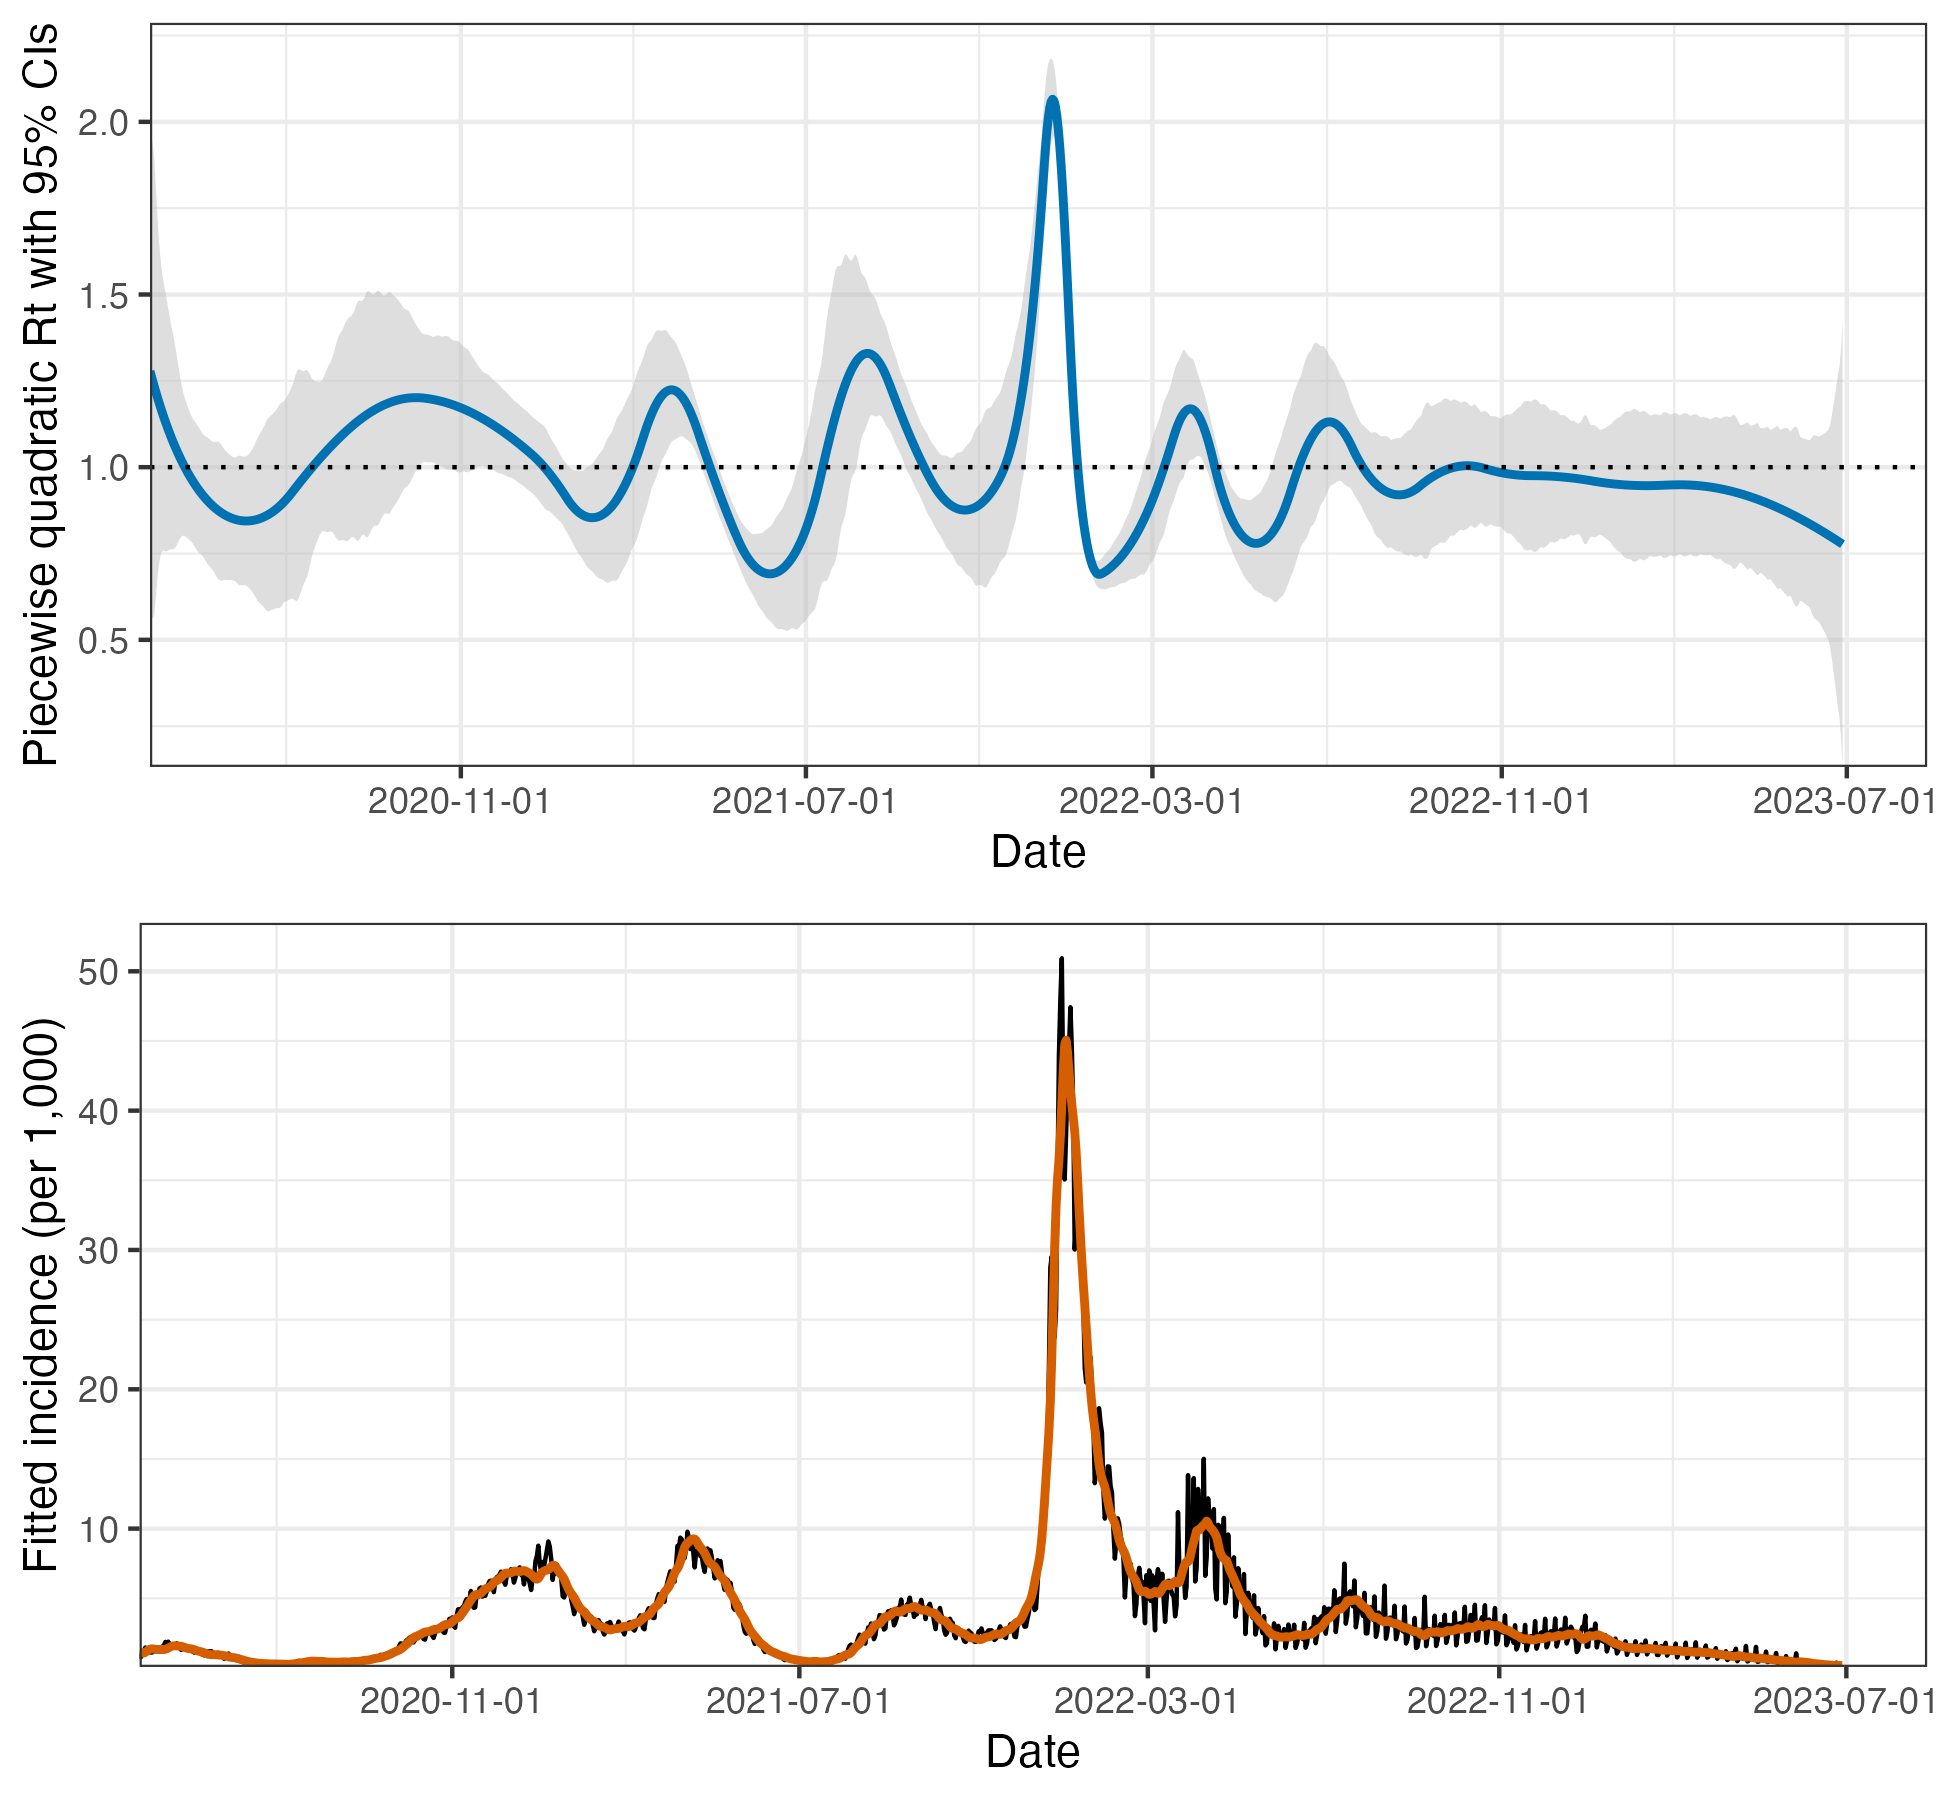
\includegraphics[width=.9\textwidth]{fig/intro-fig-new.png}
  \caption{A demonstration of effective reproduction number estimation 
  by \RtEstim\ and the corresponding predicted incident cases for the Covid-19 epidemic 
  in Canada during the period from March 28, 2020 to June 28, 2023. 
  In the top panel, the blue curve is the estimated piecewise
  quadratic $\calR_t$ and the gray ribbon is the corresponding 95\% confidence band. 
  The black curve in the bottom panel is the observed Covid-19 daily confirmed 
  cases, and the orange curve is the predicted incident cases
  corresponding to the estimated $\calR_t$.}
  \label{fig:intro-fig}
\end{figure}

While our approach is straightforward and requires little domain knowledge for
implementation, we also implement a number of refinements. 
We use a proximal Newton method to solve the convex optimization problem along
with warm starts to produce estimates efficiently, typically in a matter of 
seconds, even for long sequences of data. In a number of simulation experiments, 
we show empirically that our approach is more accurate than existing methods at 
estimating the true effective reproduction numbers. 


The manuscript proceeds as follows. We first introduce the methodology of
\RtEstim\ including the renewal equation and the development of Poisson
trend filtering estimator. We explain how this method could be interpreted from
the Bayesian perspective, connecting it to previous work in this context. We
provide illustrative experiments comparing our estimator to \EpiEstim\ and
\EpiLPS. We then apply our \RtEstim\ on the Covid-19 pandemic incidence in
British Columbia and the 1918 influenza pandemic incidence in the United States. 
Finally, we conclude with a discussion of the advantages and limitations of our 
approach and describe practical considerations for effective reproduction number
estimation.

\input{doc/Methods}
\input{doc/Results}
\input{doc/Discussion}
% Results and Discussion can be combined.


\section*{Supporting information}

% Include only the SI item label in the paragraph heading. Use the \nameref{label} command to cite SI items in the text.
\paragraph*{S1 Fig.}
\label{S1_Fig}
{\bf Covid-19 figure.} Covid-19 cases in BC and the estimated reproduction numbers.

\paragraph*{S2 Fig.}
\label{S2_Fig}
{\bf Lorem ipsum.} Maecenas convallis mauris sit amet sem ultrices gravida. Etiam eget sapien nibh. Sed ac ipsum eget enim egestas ullamcorper nec euismod ligula. Curabitur fringilla pulvinar lectus consectetur pellentesque.

\paragraph*{S1 File.}
\label{S1_File}
{\bf Lorem ipsum.}  Maecenas convallis mauris sit amet sem ultrices gravida. Etiam eget sapien nibh. Sed ac ipsum eget enim egestas ullamcorper nec euismod ligula. Curabitur fringilla pulvinar lectus consectetur pellentesque.

\paragraph*{S1 Video.}
\label{S1_Video}
{\bf Lorem ipsum.}  Maecenas convallis mauris sit amet sem ultrices gravida. Etiam eget sapien nibh. Sed ac ipsum eget enim egestas ullamcorper nec euismod ligula. Curabitur fringilla pulvinar lectus consectetur pellentesque.

\paragraph*{S1 Appendix.}
\label{S1_Appendix}
{\bf Lorem ipsum.} Maecenas convallis mauris sit amet sem ultrices gravida. Etiam eget sapien nibh. Sed ac ipsum eget enim egestas ullamcorper nec euismod ligula. Curabitur fringilla pulvinar lectus consectetur pellentesque.

\paragraph*{S1 Table.}
\label{S1_Table}
{\bf Lorem ipsum.} Maecenas convallis mauris sit amet sem ultrices gravida. Etiam eget sapien nibh. Sed ac ipsum eget enim egestas ullamcorper nec euismod ligula. Curabitur fringilla pulvinar lectus consectetur pellentesque.

\section*{Acknowledgments}
Cras egestas velit mauris, eu mollis turpis pellentesque sit amet. Interdum et malesuada fames ac ante ipsum primis in faucibus. Nam id pretium nisi. Sed ac quam id nisi malesuada congue. Sed interdum aliquet augue, at pellentesque quam rhoncus vitae.

\nolinenumbers

% Either type in your references using
% \begin{thebibliography}{}
% \bibitem{}
% Text
% \end{thebibliography}
%
% or
%
% Compile your BiBTeX database using our plos2015.bst
% style file and paste the contents of your .bbl file
% here. See http://journals.plos.org/plosone/s/latex for 
% step-by-step instructions.
% 
\begin{thebibliography}{32}
  \providecommand{\natexlab}[1]{#1}
  \providecommand{\url}[1]{\texttt{#1}}
  \expandafter\ifx\csname urlstyle\endcsname\relax
    \providecommand{\doi}[1]{doi: #1}\else
    \providecommand{\doi}{doi: \begingroup \urlstyle{rm}\Url}\fi
  
  \bibitem[Abbott et~al.(2020)Abbott, Hellewell, Thompson, Sherratt, Gibbs,
    Bosse, Munday, Meakin, Doughty, Chun, et~al.]{abbott2020estimating}
  Sam Abbott, Joel Hellewell, Robin~N Thompson, Katharine Sherratt, Hamish~P
    Gibbs, Nikos~I Bosse, James~D Munday, Sophie Meakin, Emma~L Doughty,
    June~Young Chun, et~al.
  \newblock Estimating the time-varying reproduction number of sars-cov-2 using
    national and subnational case counts.
  \newblock \emph{Wellcome Open Research}, 5\penalty0 (112):\penalty0 112, 2020.
  
  \bibitem[Abry et~al.(2020)Abry, Pustelnik, Roux, Jensen, Flandrin, Gribonval,
    Lucas, Guichard, Borgnat, and Garnier]{abry2020spatial}
  Patrice Abry, Nelly Pustelnik, St{\'e}phane Roux, Pablo Jensen, Patrick
    Flandrin, R{\'e}mi Gribonval, Charles-G{\'e}rard Lucas, {\'E}ric Guichard,
    Pierre Borgnat, and Nicolas Garnier.
  \newblock Spatial and temporal regularization to estimate covid-19 reproduction
    number r (t): Promoting piecewise smoothness via convex optimization.
  \newblock \emph{Plos one}, 15\penalty0 (8):\penalty0 e0237901, 2020.
  
  \bibitem[Alene et~al.(2021)Alene, Yismaw, Assemie, Ketema, Gietaneh, and
    Birhan]{alene2021serial}
  Muluneh Alene, Leltework Yismaw, Moges~Agazhe Assemie, Daniel~Bekele Ketema,
    Wodaje Gietaneh, and Tilahun~Yemanu Birhan.
  \newblock Serial interval and incubation period of covid-19: a systematic
    review and meta-analysis.
  \newblock \emph{BMC Infectious Diseases}, 21:\penalty0 1--9, 2021.
  
  \bibitem[Azmon et~al.(2014)Azmon, Faes, and Hens]{azmon2014estimation}
  Amin Azmon, Christel Faes, and Niel Hens.
  \newblock On the estimation of the reproduction number based on misreported
    epidemic data.
  \newblock \emph{Statistics in medicine}, 33\penalty0 (7):\penalty0 1176--1192,
    2014.
  
  \bibitem[Bo{\"e}lle et~al.(2011)Bo{\"e}lle, Ansart, Cori, and
    Valleron]{boelle2011transmission}
  Pierre-Yves Bo{\"e}lle, Severine Ansart, Anne Cori, and Alain-Jacques Valleron.
  \newblock Transmission parameters of the a/h1n1 (2009) influenza virus
    pandemic: a review.
  \newblock \emph{Influenza and other respiratory viruses}, 5\penalty0
    (5):\penalty0 306--316, 2011.
  
  \bibitem[Brauer et~al.(2019)Brauer, Castillo-Chavez, and
    Feng]{brauer2019mathematical}
  Fred Brauer, Carlos Castillo-Chavez, and Zhilan Feng.
  \newblock \emph{Mathematical models in epidemiology}, volume~32.
  \newblock Springer, 2019.
  
  \bibitem[Cori et~al.(2013)Cori, Ferguson, Fraser, and Cauchemez]{cori2013new}
  Anne Cori, Neil~M Ferguson, Christophe Fraser, and Simon Cauchemez.
  \newblock A new framework and software to estimate time-varying reproduction
    numbers during epidemics.
  \newblock \emph{American journal of epidemiology}, 178\penalty0 (9):\penalty0
    1505--1512, 2013.
  
  \bibitem[Cori et~al.(2020)Cori, Cauchemez, Ferguson, Fraser, Dahlqwist,
    Demarsh, Jombart, Kamvar, Lessler, Li, et~al.]{cori2020package}
  Anne Cori, Simon Cauchemez, Neil~M Ferguson, Christophe Fraser, Elisabeth
    Dahlqwist, P~Alex Demarsh, Thibaut Jombart, Zhian~N Kamvar, Justin Lessler,
    Shikun Li, et~al.
  \newblock Package `epiestim'.
  \newblock \emph{CRAN: Vienna Austria}, 2020.
  
  \bibitem[Gressani et~al.(2021)Gressani, Faes, and
    Hens]{gressani2021approximate}
  Oswaldo Gressani, Christel Faes, and Niel Hens.
  \newblock An approximate bayesian approach for estimation of the reproduction
    number under misreported epidemic data.
  \newblock \emph{MedRxiv}, pages 2021--05, 2021.
  
  \bibitem[Gressani et~al.(2022)Gressani, Wallinga, Althaus, Hens, and
    Faes]{gressani2022epilps}
  Oswaldo Gressani, Jacco Wallinga, Christian~L Althaus, Niel Hens, and Christel
    Faes.
  \newblock Epilps: A fast and flexible bayesian tool for estimation of the
    time-varying reproduction number.
  \newblock \emph{PLoS computational biology}, 18\penalty0 (10):\penalty0
    e1010618, 2022.
  
  \bibitem[Griffin et~al.(2020)Griffin, Casey, Collins, Hunt, McEvoy, Byrne,
    McAloon, Barber, Lane, and More]{griffin2020rapid}
  John Griffin, Miriam Casey, {\'A}ine Collins, Kevin Hunt, David McEvoy, Andrew
    Byrne, Conor McAloon, Ann Barber, Elizabeth~Ann Lane, and SImon More.
  \newblock Rapid review of available evidence on the serial interval and
    generation time of covid-19.
  \newblock \emph{BMJ open}, 10\penalty0 (11):\penalty0 e040263, 2020.
  
  \bibitem[Hettinger et~al.(2023)Hettinger, Rubin, and
    Huang]{hettinger2023estimating}
  Gary Hettinger, David Rubin, and Jing Huang.
  \newblock Estimating the instantaneous reproduction number with imperfect data:
    A method to account for case-reporting variation and serial interval
    uncertainty.
  \newblock \emph{arXiv preprint arXiv:2302.12078}, 2023.
  
  \bibitem[Ho et~al.(2023)Ho, Parag, Adam, Lau, Cowling, and
    Tsang]{ho2023accounting}
  Faith Ho, Kris~V Parag, Dillon~C Adam, Eric~HY Lau, Benjamin~J Cowling, and
    Tim~K Tsang.
  \newblock Accounting for the potential of overdispersion in estimation of the
    time-varying reproduction number.
  \newblock \emph{Epidemiology}, 34\penalty0 (2):\penalty0 201--205, 2023.
  
  \bibitem[Jin et~al.(2023)Jin, Dickens, Lim, and Cook]{jin2023epimix}
  Shihui Jin, Borame~Lee Dickens, Jue~Tao Lim, and Alex~R Cook.
  \newblock Epimix: A novel method to estimate effective reproduction number.
  \newblock \emph{Infectious Disease Modelling}, 2023.
  
  \bibitem[Johnson(2013)]{johnson2013dynamic}
  Nicholas~A Johnson.
  \newblock A dynamic programming algorithm for the fused lasso and
    $\ell_0$-segmentation.
  \newblock \emph{Journal of Computational and Graphical Statistics}, 22\penalty0
    (2):\penalty0 246--260, 2013.
  
  \bibitem[Kim et~al.(2009)Kim, Koh, Boyd, and Gorinevsky]{kim2009ell_1}
  Seung-Jean Kim, Kwangmoo Koh, Stephen Boyd, and Dimitry Gorinevsky.
  \newblock $\ell_1$ trend filtering.
  \newblock \emph{SIAM review}, 51\penalty0 (2):\penalty0 339--360, 2009.
  
  \bibitem[Lison et~al.(2023)Lison, Abbott, Huisman, and
    Stadler]{lison2023generative}
  Adrian Lison, Sam Abbott, Jana Huisman, and Tanja Stadler.
  \newblock Generative bayesian modeling to nowcast the effective reproduction
    number from line list data with missing symptom onset dates.
  \newblock \emph{arXiv preprint arXiv:2308.13262}, 2023.
  
  \bibitem[Nash et~al.(2023)Nash, Bhatt, Cori, and Nouvellet]{nash2023estimating}
  Rebecca~K Nash, Samir Bhatt, Anne Cori, and Pierre Nouvellet.
  \newblock Estimating the epidemic reproduction number from temporally
    aggregated incidence data: A statistical modelling approach and software
    tool.
  \newblock \emph{PLOS Computational Biology}, 19\penalty0 (8):\penalty0
    e1011439, 2023.
  
  \bibitem[Parag(2021)]{parag2021improved}
  Kris~V Parag.
  \newblock Improved estimation of time-varying reproduction numbers at low case
    incidence and between epidemic waves.
  \newblock \emph{PLoS Computational Biology}, 17\penalty0 (9):\penalty0
    e1009347, 2021.
  
  \bibitem[Pascal et~al.(2022)Pascal, Abry, Pustelnik, Roux, Gribonval, and
    Flandrin]{pascal2022nonsmooth}
  Barbara Pascal, Patrice Abry, Nelly Pustelnik, St{\'e}phane Roux, R{\'e}mi
    Gribonval, and Patrick Flandrin.
  \newblock Nonsmooth convex optimization to estimate the covid-19 reproduction
    number space-time evolution with robustness against low quality data.
  \newblock \emph{IEEE Transactions on Signal Processing}, 70:\penalty0
    2859--2868, 2022.
  
  \bibitem[Pircalabelu(2023{\natexlab{a}})]{pircal2023spline}
  Eugen Pircalabelu.
  \newblock A spline-based time-varying reproduction number for modelling
    epidemiological outbreaks.
  \newblock \emph{Journal of the Royal Statistical Society Series C: Applied
    Statistics}, page qlad027, 2023{\natexlab{a}}.
  
  \bibitem[Pircalabelu(2023{\natexlab{b}})]{pircalabelu2023spline}
  Eugen Pircalabelu.
  \newblock A spline-based time-varying reproduction number for modelling
    epidemiological outbreaks.
  \newblock \emph{Journal of the Royal Statistical Society Series C: Applied
    Statistics}, page qlad027, 2023{\natexlab{b}}.
  
  \bibitem[Rai et~al.(2021)Rai, Shukla, and Dwivedi]{rai2021estimates}
  Balram Rai, Anandi Shukla, and Laxmi~Kant Dwivedi.
  \newblock Estimates of serial interval for covid-19: A systematic review and
    meta-analysis.
  \newblock \emph{Clinical epidemiology and global health}, 9:\penalty0 157--161,
    2021.
  
  \bibitem[Ramdas and Tibshirani(2016)]{ramdas2016fast}
  Aaditya Ramdas and Ryan~J Tibshirani.
  \newblock Fast and flexible admm algorithms for trend filtering.
  \newblock \emph{Journal of Computational and Graphical Statistics}, 25\penalty0
    (3):\penalty0 839--858, 2016.
  
  \bibitem[Sadhanala et~al.(2022)Sadhanala, Bassett, Sharpnack, and
    McDonald]{sadhanala2022exponential}
  Veeranjaneyulu Sadhanala, Robert Bassett, James Sharpnack, and Daniel~J
    McDonald.
  \newblock Exponential family trend filtering on lattices.
  \newblock \emph{arXiv preprint arXiv:2209.09175}, 2022.
  
  \bibitem[{Sam Abbott} et~al.(2020){Sam Abbott}, {Joel Hellewell}, {Katharine
    Sherratt}, {Katelyn Gostic}, {Joe Hickson}, {Hamada S. Badr}, {Michael
    DeWitt}, {Robin Thompson}, {EpiForecasts}, and {Sebastian Funk}]{EpiNow2}
  {Sam Abbott}, {Joel Hellewell}, {Katharine Sherratt}, {Katelyn Gostic}, {Joe
    Hickson}, {Hamada S. Badr}, {Michael DeWitt}, {Robin Thompson},
    {EpiForecasts}, and {Sebastian Funk}.
  \newblock \emph{EpiNow2: Estimate Real-Time Case Counts and Time-Varying
    Epidemiological Parameters}, 2020.
  
  \bibitem[Taubenberger and Morens(2006)]{taubenberger20061918}
  Jeffery~K Taubenberger and David~M Morens.
  \newblock 1918 influenza: the mother of all pandemics.
  \newblock \emph{Revista Biomedica}, 17\penalty0 (1):\penalty0 69--79, 2006.
  
  \bibitem[Thompson et~al.(2019)Thompson, Stockwin, van Gaalen, Polonsky, Kamvar,
    Demarsh, Dahlqwist, Li, Miguel, Jombart, et~al.]{thompson2019improved}
  Robin~N Thompson, Jake~E Stockwin, Rolina~D van Gaalen, Jonny~A Polonsky,
    Zhian~N Kamvar, P~Alex Demarsh, Elisabeth Dahlqwist, Siyang Li, Eve Miguel,
    Thibaut Jombart, et~al.
  \newblock Improved inference of time-varying reproduction numbers during
    infectious disease outbreaks.
  \newblock \emph{Epidemics}, 29:\penalty0 100356, 2019.
  
  \bibitem[Tibshirani(2014)]{tibshirani2014adaptive}
  Ryan~J Tibshirani.
  \newblock Adaptive piecewise polynomial estimation via trend filtering.
  \newblock \emph{The Annals of Statistics}, 42\penalty0 (1):\penalty0 285--323,
    2014.
  
  \bibitem[Tibshirani et~al.(2022)]{tibshirani2022divided}
  Ryan~J Tibshirani et~al.
  \newblock Divided differences, falling factorials, and discrete splines:
    Another look at trend filtering and related problems.
  \newblock \emph{Foundations and Trends{\textregistered} in Machine Learning},
    15\penalty0 (6):\penalty0 694--846, 2022.
  
  \bibitem[Trevisin et~al.(2023)Trevisin, Bertuzzo, Pasetto, Mari, Miccoli,
    Casagrandi, Gatto, and Rinaldo]{trevisin2023spatially}
  Cristiano Trevisin, Enrico Bertuzzo, Damiano Pasetto, Lorenzo Mari, Stefano
    Miccoli, Renato Casagrandi, Marino Gatto, and Andrea Rinaldo.
  \newblock Spatially explicit effective reproduction numbers from incidence and
    mobility data.
  \newblock \emph{Proceedings of the National Academy of Sciences}, 120\penalty0
    (20):\penalty0 e2219816120, 2023.
  
  \bibitem[White et~al.(2009)White, Wallinga, Finelli, Reed, Riley, Lipsitch, and
    Pagano]{white2009estimation}
  Laura~Forsberg White, Jacco Wallinga, Lyn Finelli, Carrie Reed, Steven Riley,
    Marc Lipsitch, and Marcello Pagano.
  \newblock Estimation of the reproductive number and the serial interval in
    early phase of the 2009 influenza a/h1n1 pandemic in the usa.
  \newblock \emph{Influenza and other respiratory viruses}, 3\penalty0
    (6):\penalty0 267--276, 2009.
  
  \end{thebibliography}

  
%\bibliography{ptf}

\end{document}
